Cette section va établir que, relativement au problème d'isopérimétrie polygonal,
un \ngone\ solution doit être convexe, 
puis
qu'un \ngone\ convexe solution doit être un \nreg,
et enfin
que si $\setproba*{R}{1}$ et $\setproba*{R}{2}$ sont respectivement un \xgone{k_1} et un \xgone{k_2}, tous les deux réguliers convexes, avec 
$k_1 < k_2$ et $\perim{\setproba*{R}{1}} = \perim{\setproba*{R}{2}}$, 
alors
$\area{\setproba*{R}{1}} < \area{\setproba*{R}{2}}$.
Nous pourrons alors conclure dans la section finale suivante.


\begin{tcolorbox}
	\itshape\small
	Les cas $n = 3$ et $n = 4$ étant résolus, voir les faits \ref{iso-tri} et \ref{quadri}, dans toutes les preuves de cette section, nous supposerons $n \geq 5$.
\end{tcolorbox}


% ----------------------- %


\begin{fact} \label{must-be-conv}
    Pour tout \ngone\ non convexe $\setproba{P}$, alors on peut construire un \ngone\ convexe $\setproba{C}$ tel que
	$\perim{\setproba{C}} = \perim{\setproba{P}}$
	et
	$\area{\setproba{C}} > \area{\setproba{P}}$.
\end{fact}


\begin{proof}
	Soit $\setproba{E}$ l'enveloppe convexe d'un \ngone\ non convexe $\setproba{P}$ (voir ci-dessous).
	
	\begin{center}
		\centering
		\small\itshape
		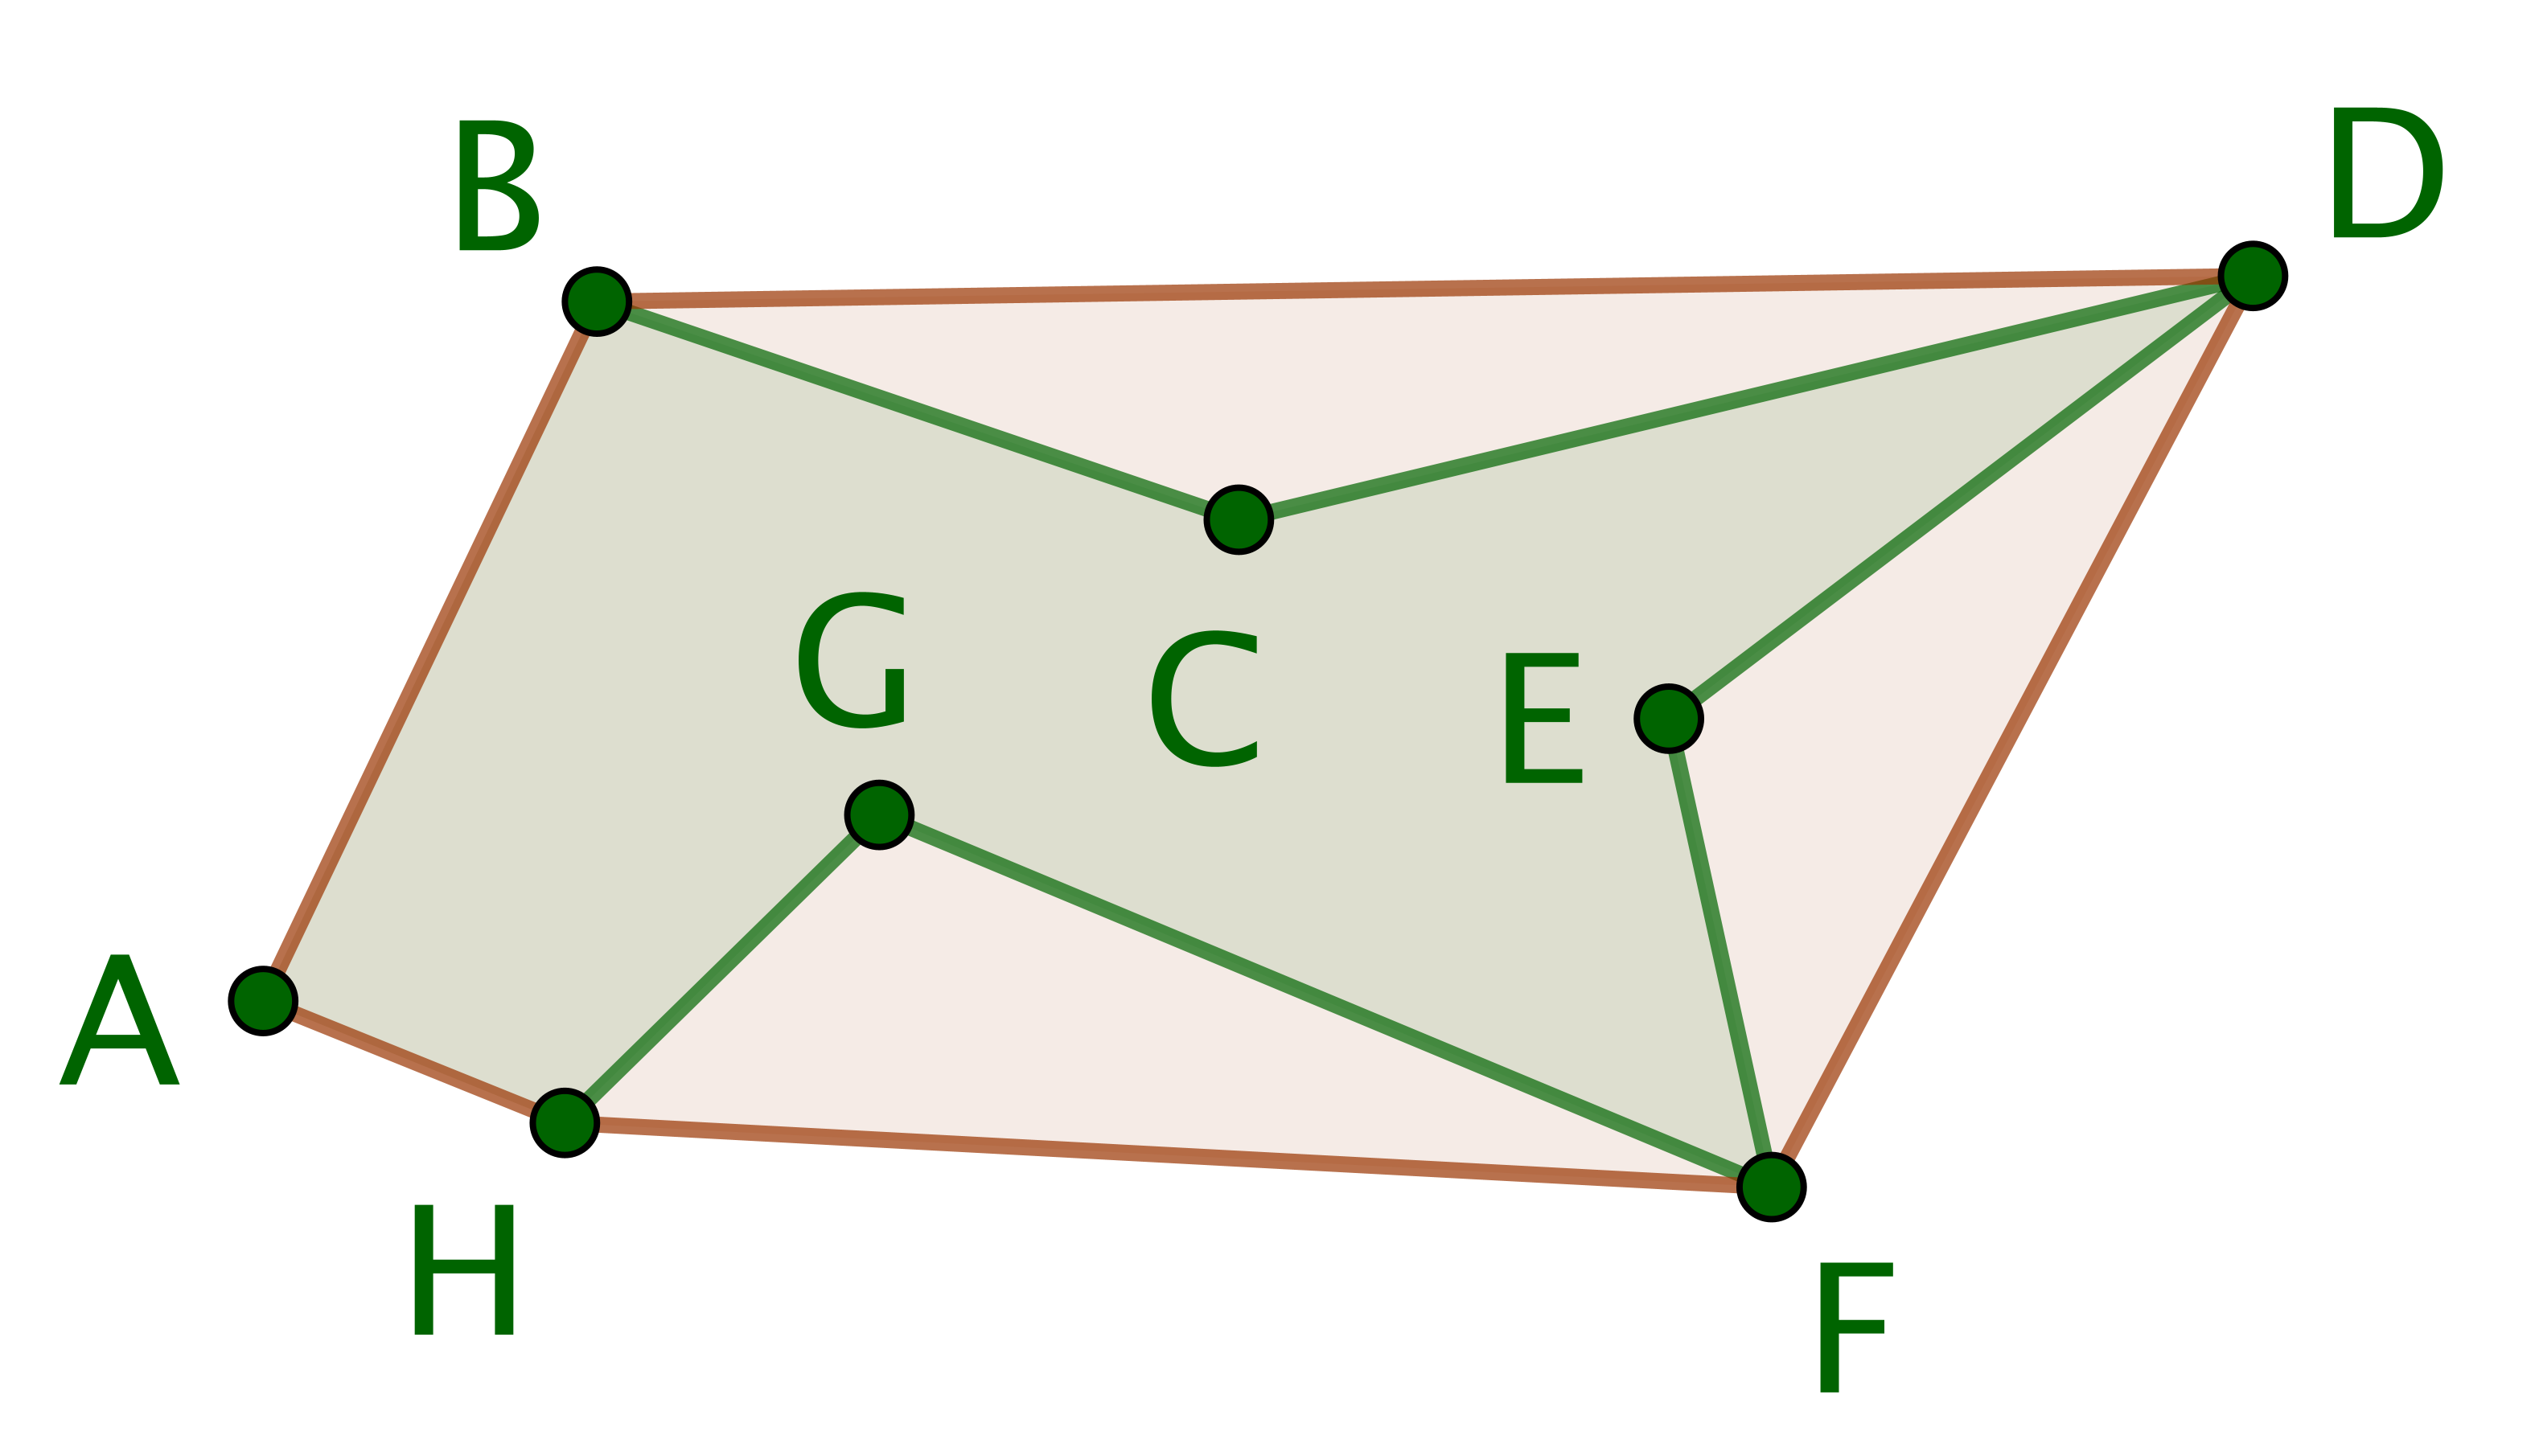
\includegraphics[scale=.45]{content/polygon/sol-must-be/convex-hull.png}
	\end{center}
	
		
	Clairement,
	$\perim{\setproba{E}} < \perim{\setproba{P}}$
	et
	$\area{\setproba{E}} > \area{\setproba{P}}$,
	mais
	$\setproba{E}$ est un \xgone{s} avec $s < n$. 
	%
	Pour gérer ce problème, une idée simple, formalisée après, est d'ajouter des sommets assez prêts des côtés de $\setproba{E}$ pour garder 
	la convexité, 
	un périmètre inférieur à $\perim{\setproba{P}}$, 
	et
	une aire supérieure à $\area{\setproba{P}}$.
	Si c'est faisable, une homothétie de rapport $r \geq 1$, où $r = \frac{ \perim{\setproba{P}} }{ \perim{\setproba{E}} }$, donnera le \ngone\ convexe $\setproba{C}$ cherché.
	La figure suivante illustre cette idée.
	
	\begin{center}
		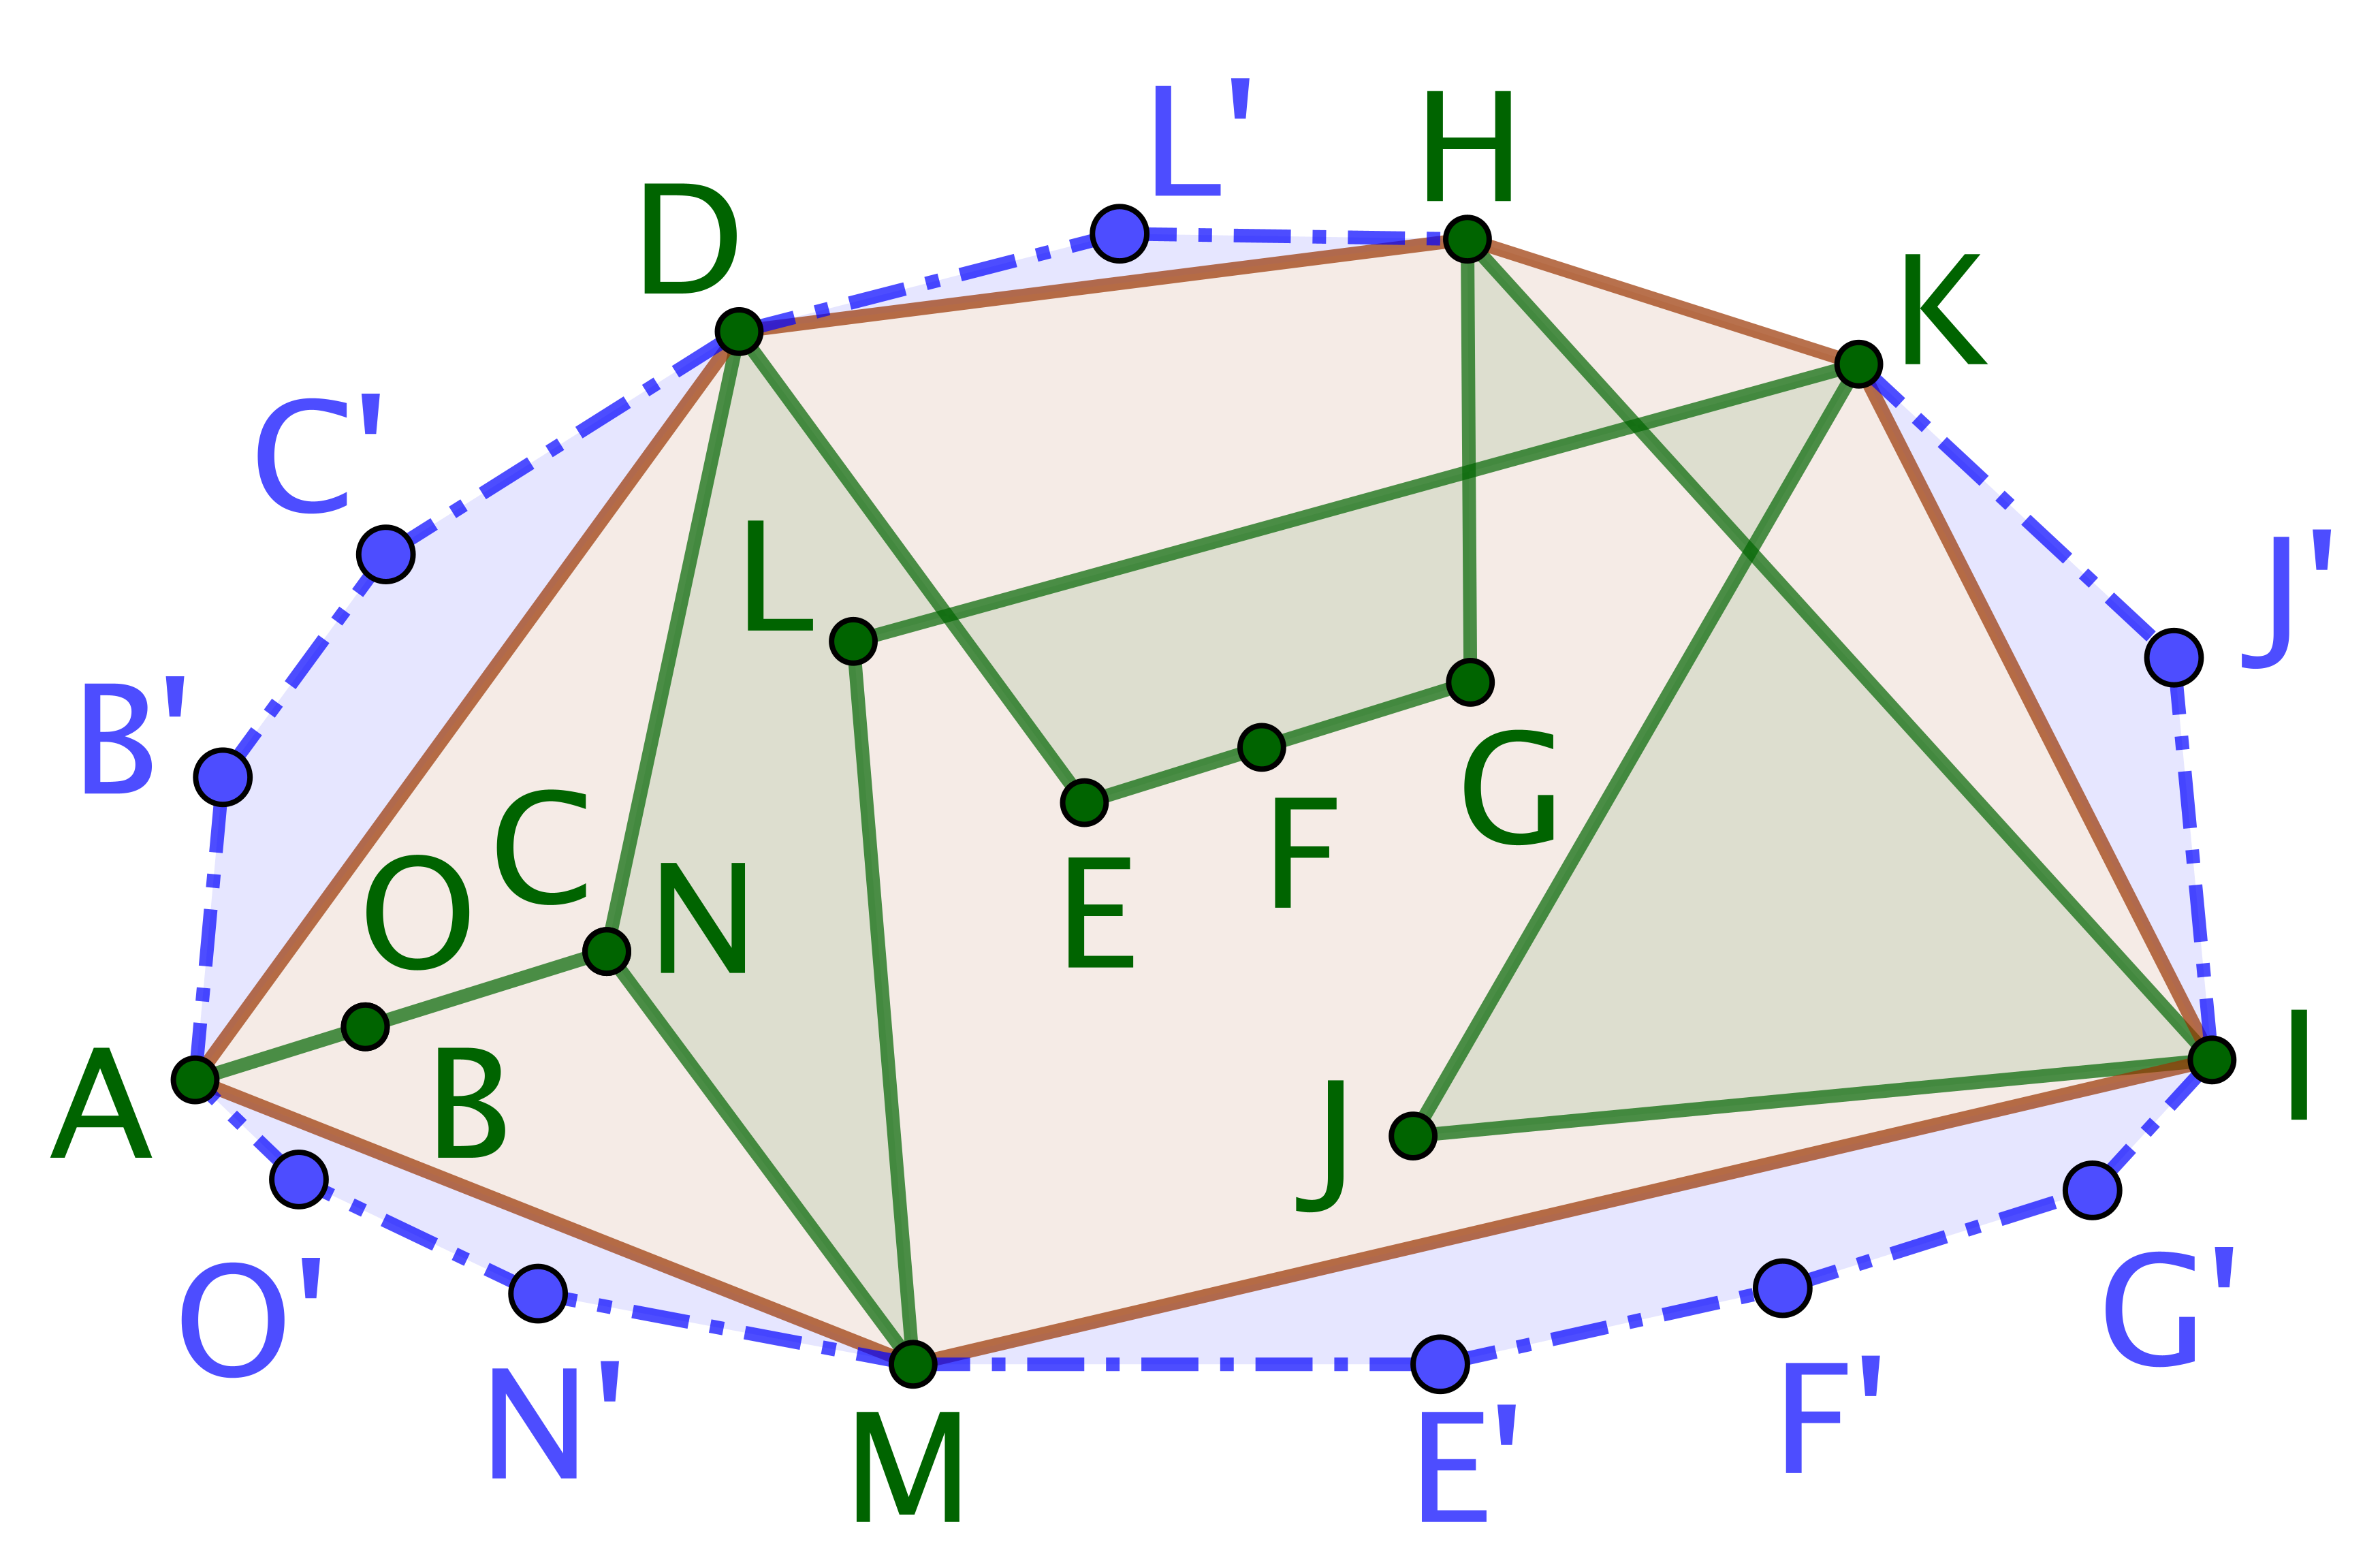
\includegraphics[scale=.45]{content/polygon/sol-must-be/convex-hull-distortion.png}
	\end{center}

	\newpage % TEMPO

	Notons $m = n - s$ qui compte les sommets manquants, puis posons
	$\delta = \frac{\perim{\setproba{P}} - \perim{\setproba{E}}}{m}$.
	%
	\begin{enumerate}
		\item \label{add-vertex-start}
		Considérons $[AB]$ un côté quelconque de $\setproba{E}$.
		Les droites portées par les côtés \focus{autour} de $[AB]$ \focus{dessinent} une région contenant toujours un triangle $ABC$ dont l'intérieur est à l'extérieur
		\footnote{
			C'est ce que l'on appelle de la \focus{low poetry},.
		}
		de $\setproba{E}$ comme dans les deux cas ci-dessous.
	%
		\begin{multicols}{2}
			\centering

			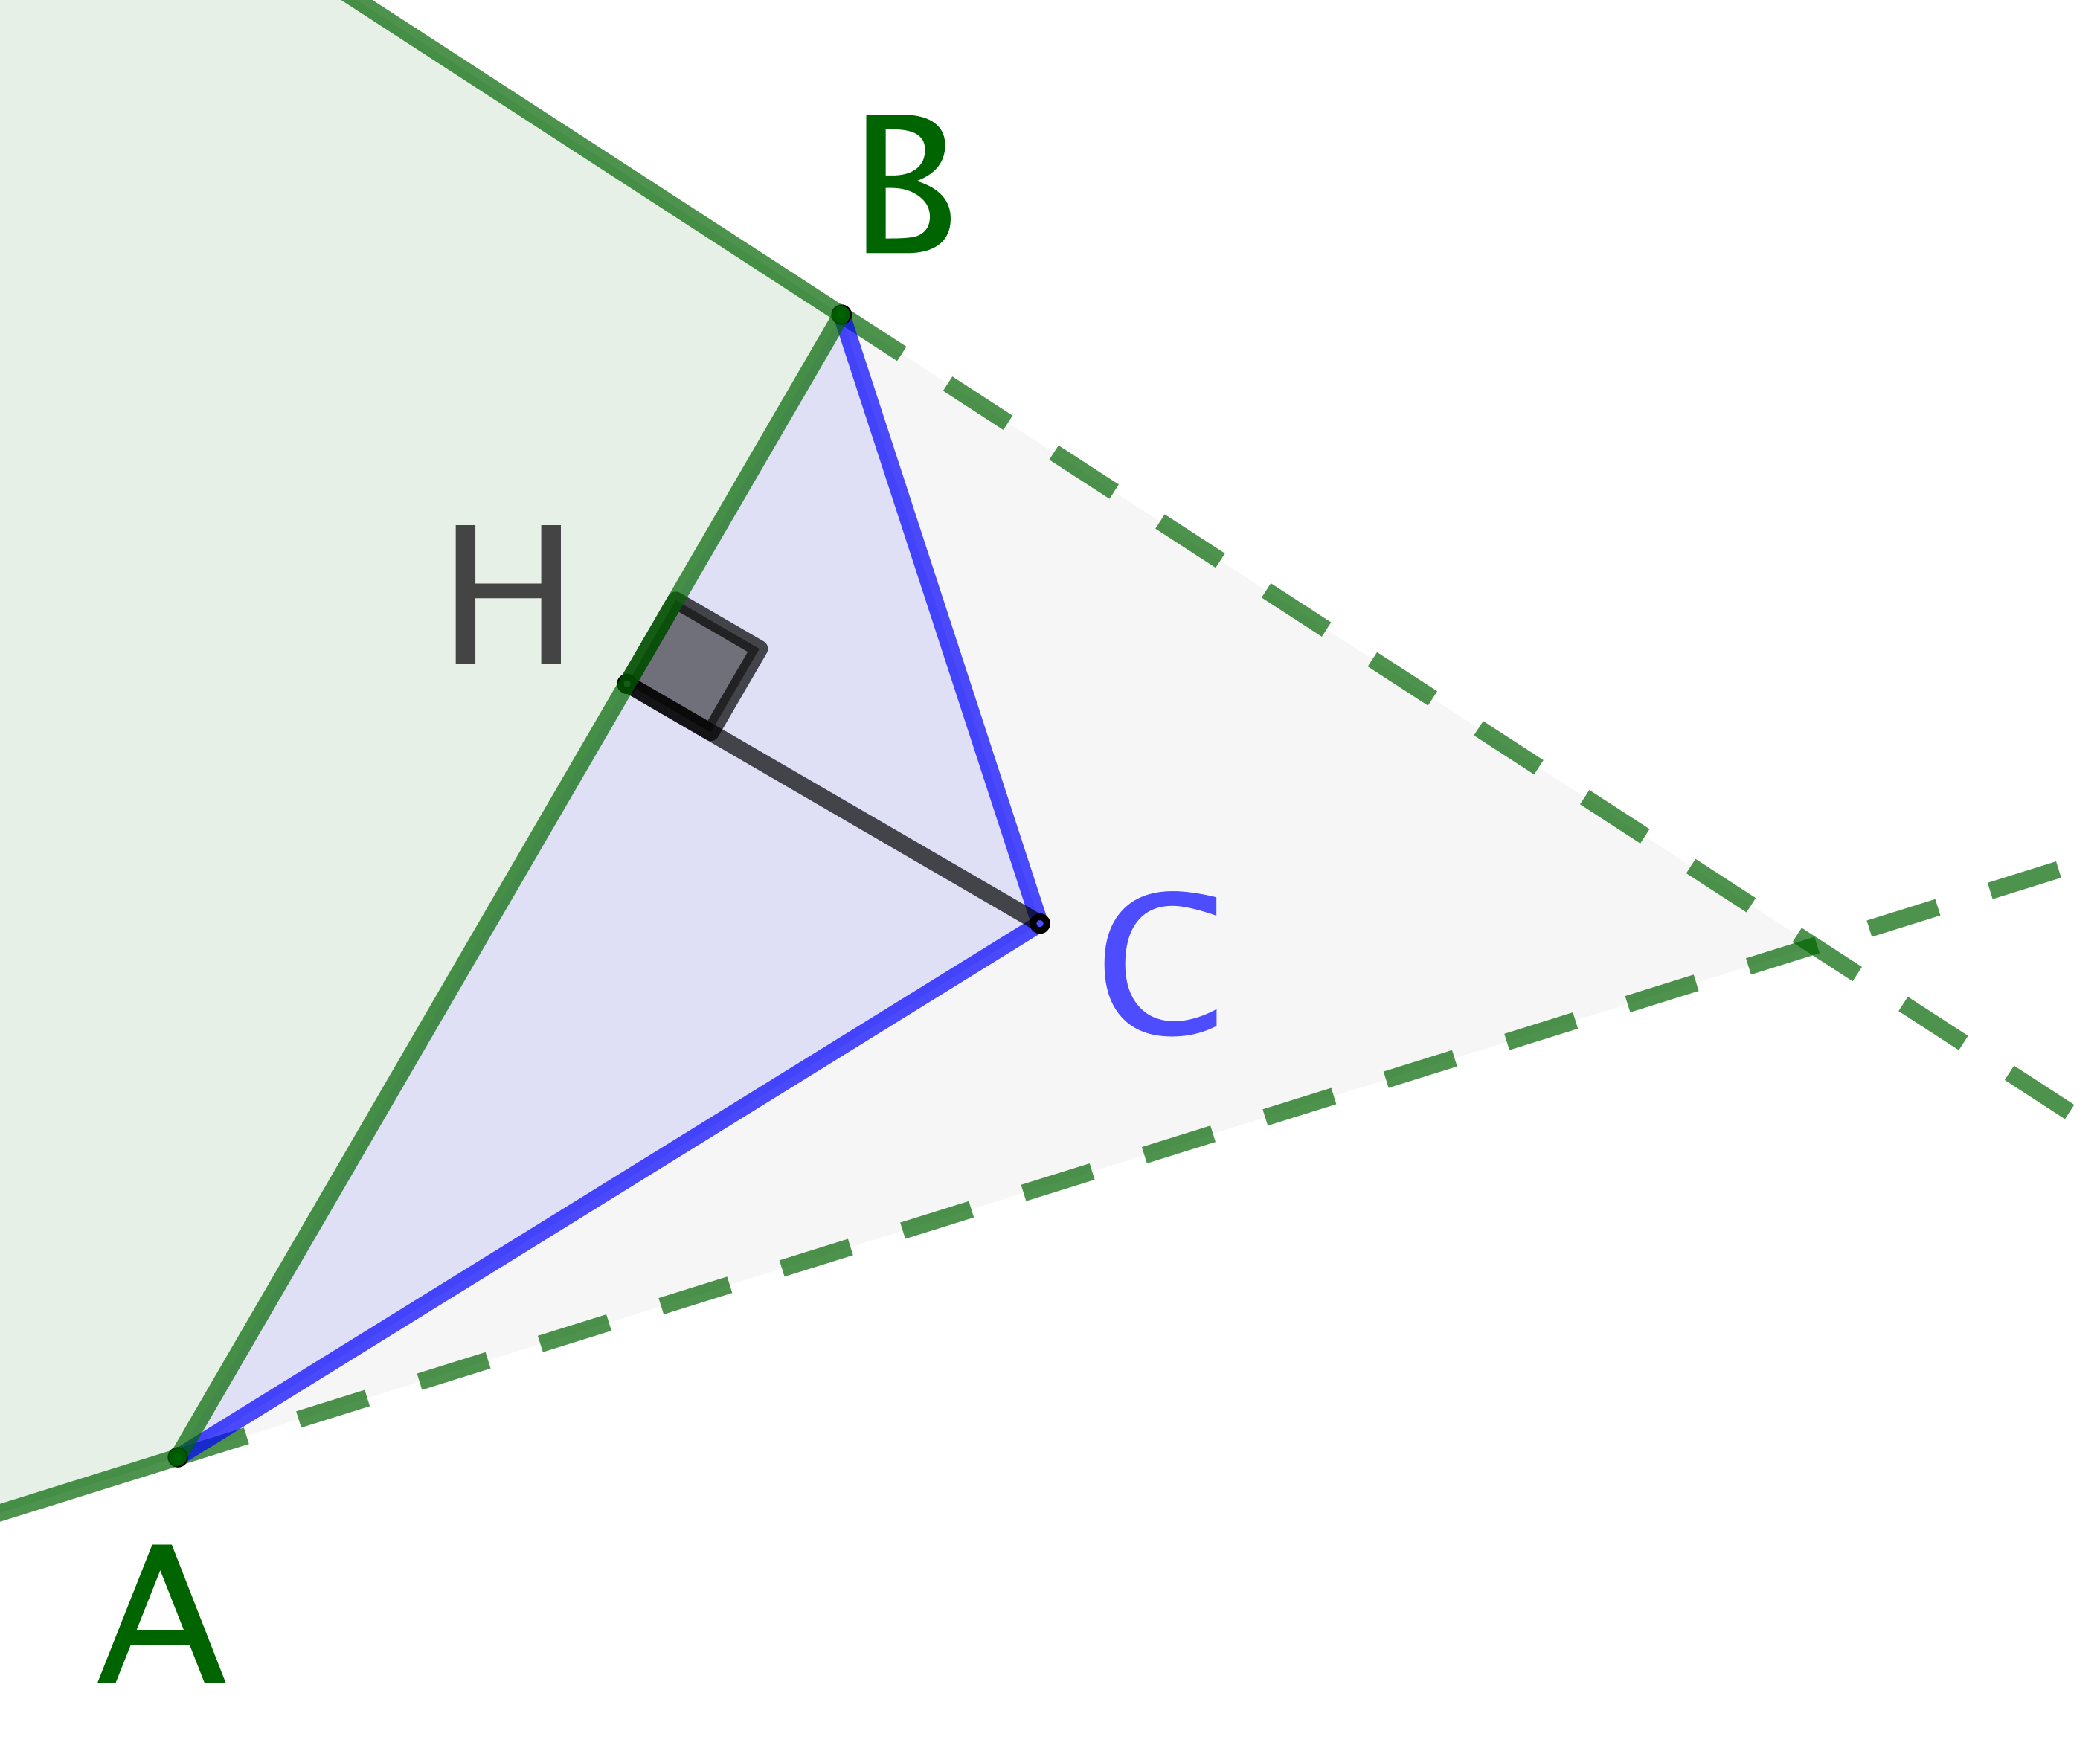
\includegraphics[scale=.35]{content/polygon/sol-must-be/add-vertex-1.png}

			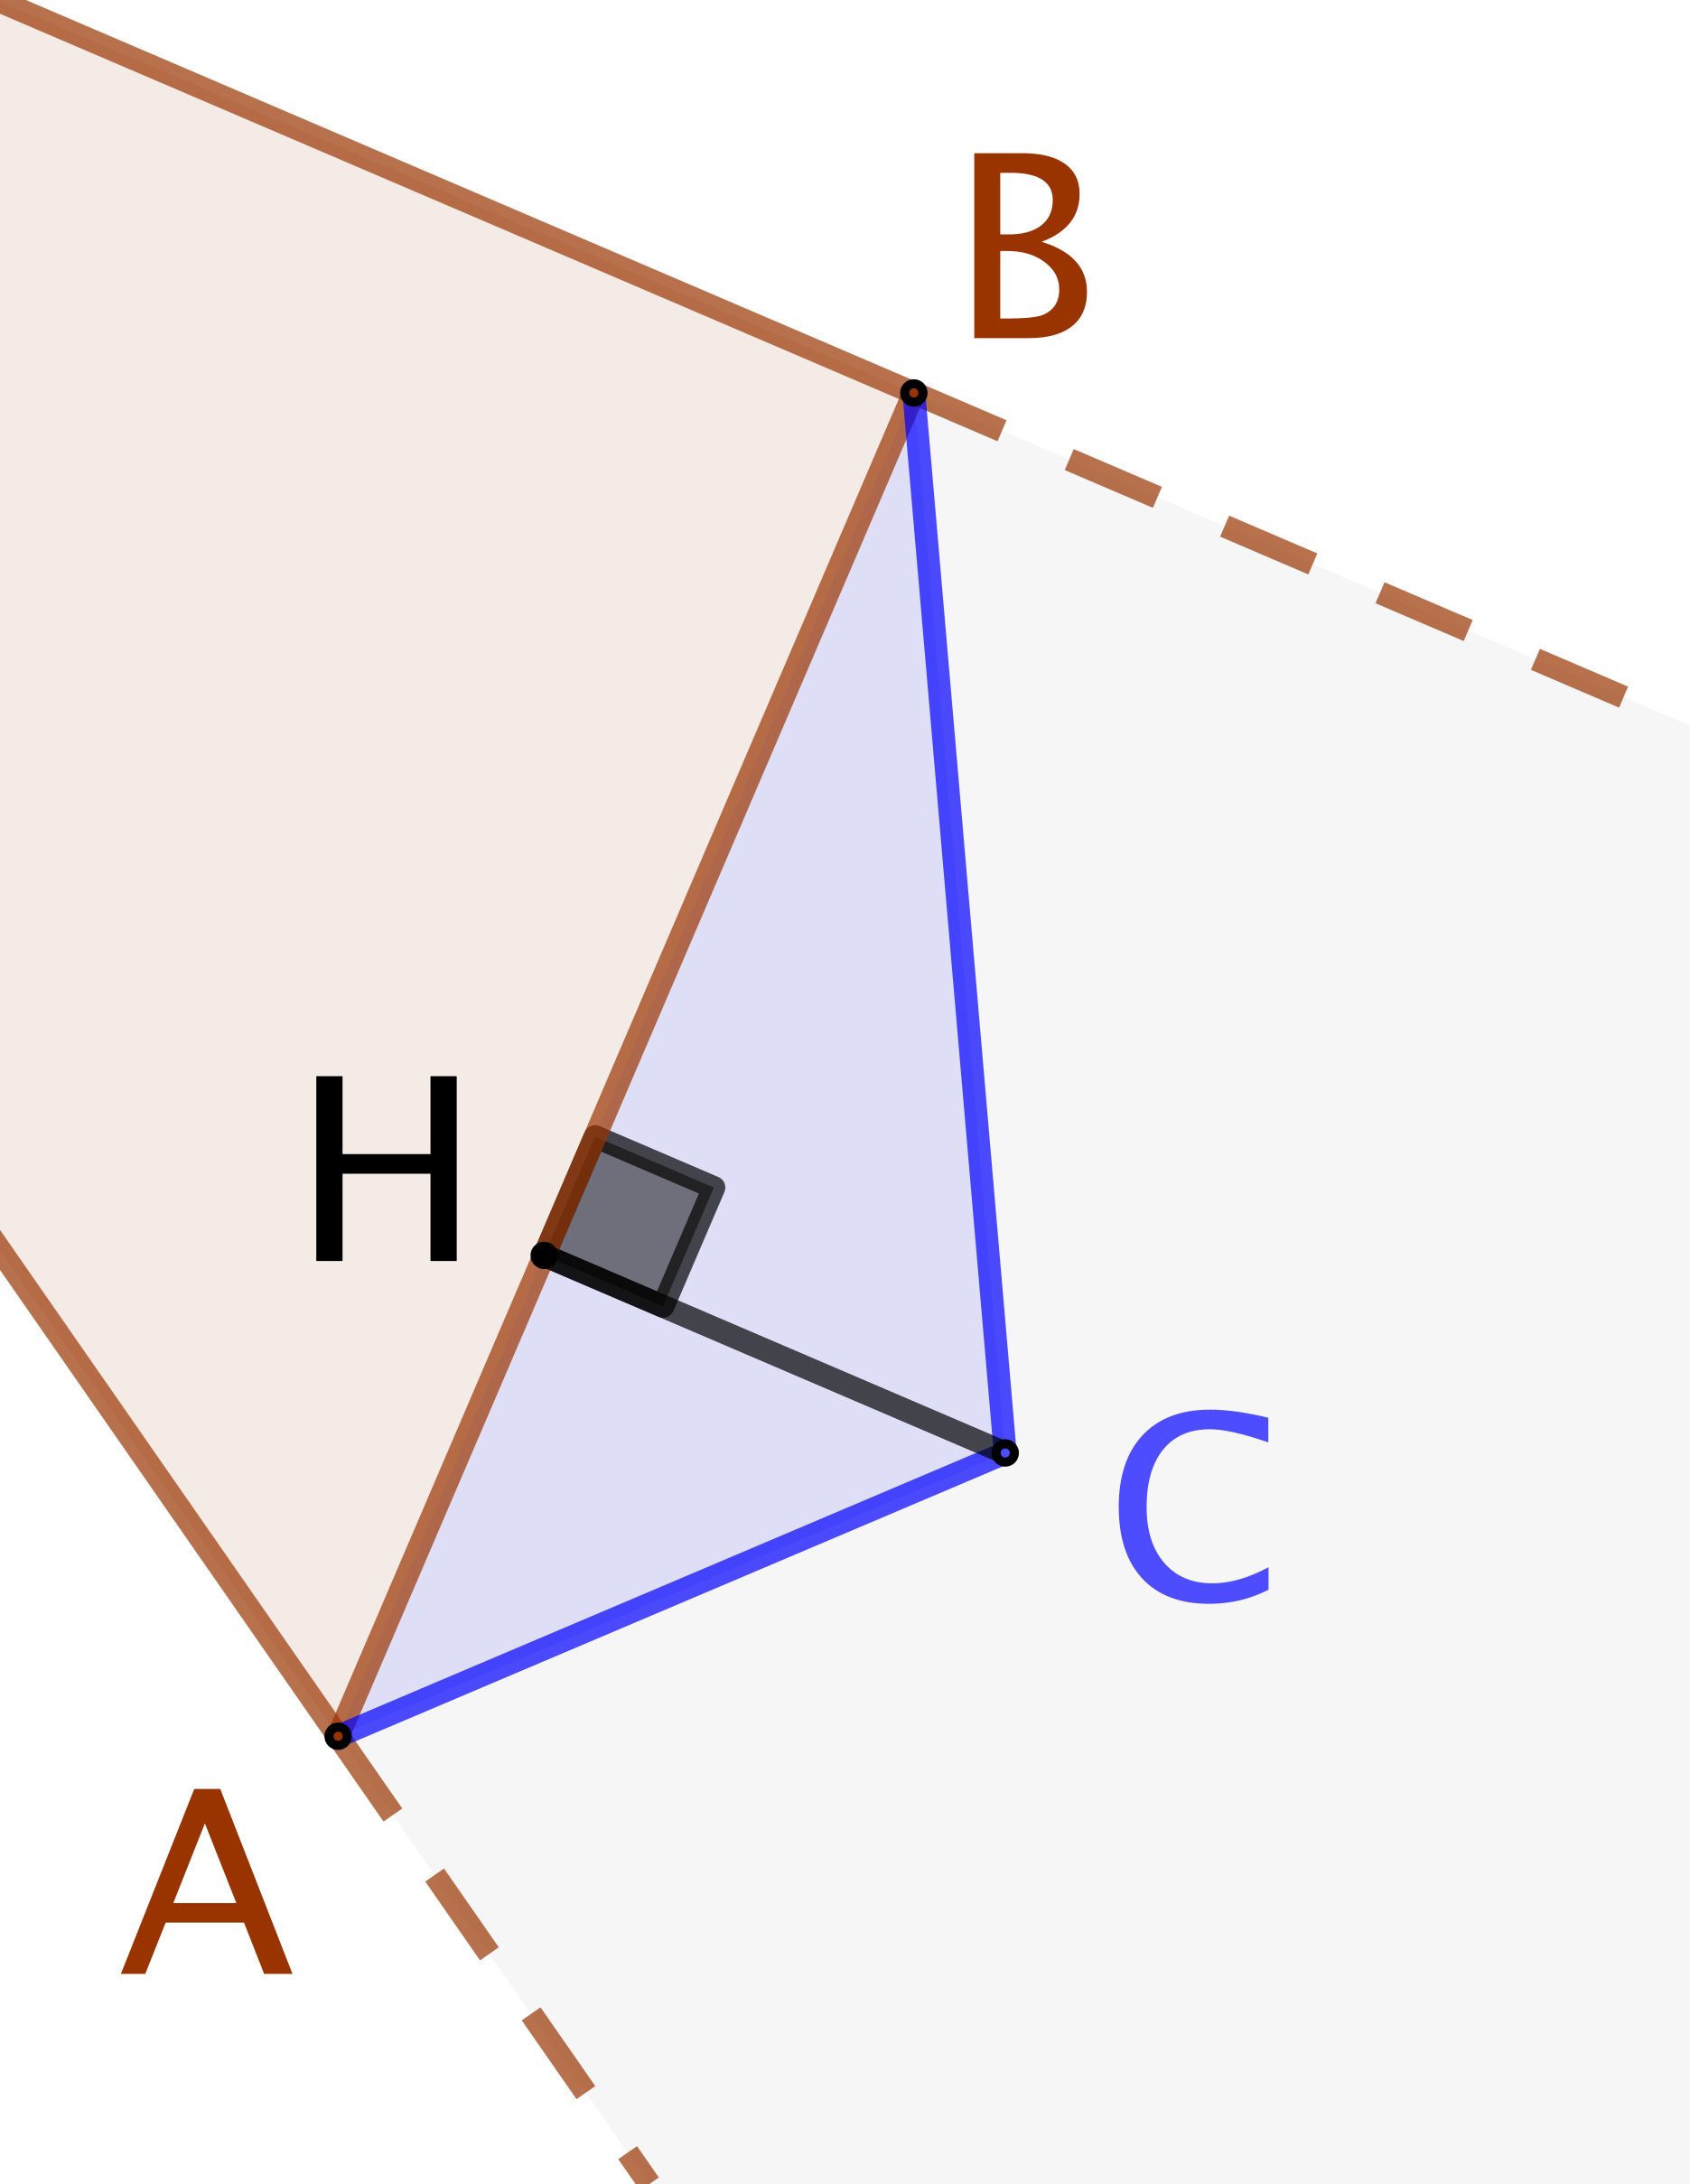
\includegraphics[scale=.35]{content/polygon/sol-must-be/add-vertex-2.png}
		\end{multicols}

		\item Clairement, le polygone $\setproba{E}_+$ obtenu à partir de $\setproba{E}$ en remplaçant le côté $[AB]$ par les côtés $[AC]$ et $[CB]$ est un convexe avec un sommet de plus que $\setproba{E}$.

		\item \label{add-vertex-end}
		Comme $HC$ peut être rendu aussi proche de $0$ que souhaité, il est aisé de voir que l'on peut choisir cette distance de sorte que $AC + BC < AB + \delta$.
		Dès lors, le périmètre de $\setproba{E}_+$ augmente inférieurement strictement à $\delta$ relativement à $\setproba{E}$.

		\item En répétant $(m-1)$ fois les étapes \ref{add-vertex-start} à \ref{add-vertex-end}, nous obtenons un \ngone\ convexe $\setproba{C}$ tel que
		$\area{\setproba{C}} > \area{\setproba{P}}$
		et
		$\perim{\setproba{C}} < \perim{\setproba{E}} + m \delta = \perim{\setproba{P}}$.
	\end{enumerate}
	
	\null\vspace{-6ex}
\end{proof}


% ----------------------- %


\begin{fact} \label{must-be-equi}
	Si un \ngone\ convexe $\setproba{P}$ n'est pas équilatéral, alors on peut construire un \ngone\ convexe $\primeit{\setproba{P}}$ tel que
	$\perim{\primeit{\setproba{P}}} = \perim{\setproba{P}}$
	et
	$\area{\primeit{\setproba{P}}} > \area{\setproba{P}}$.
\end{fact}


\begin{proof}
	Considérons un \ngone\ convexe non équilatéral $\setproba{P}$.
	%
	Dans ce cas, $\setproba{P}$ admet un triplet de sommets consécutifs $A$, $B$ et $C$ tels que $AB \neq BC$
	(sinon, on obtiendrait de proche en proche l'équilatéralité).
	La construction vue dans la preuve du fait \ref{tri-one-side-fixed} nous donne la solution: voir les deux dessins ci-après dans lesquels $(AC) \parallel (BB^{\,\prime})$.
	Pour le 2\ieme\ cas, il n'est pas possible d'utiliser le triangle $AB^{\,\prime}C$ isocèle en $B^{\,\prime}$ car $(B^{\,\prime}C)$ porte le côté de $\setproba{P}$ de sommet $C$ juste après $[BC]$, mais ce problème se contourne en considérant un point $B^{\,\prime\prime}$ du segment ouvert $]BB^{\,\prime}[$ (si besoin, se reporter au 2\ieme\ dessin de la preuve du fait \ref{tri-one-side-fixed}).
	%
	\begin{multicols}{2}
		\centering

		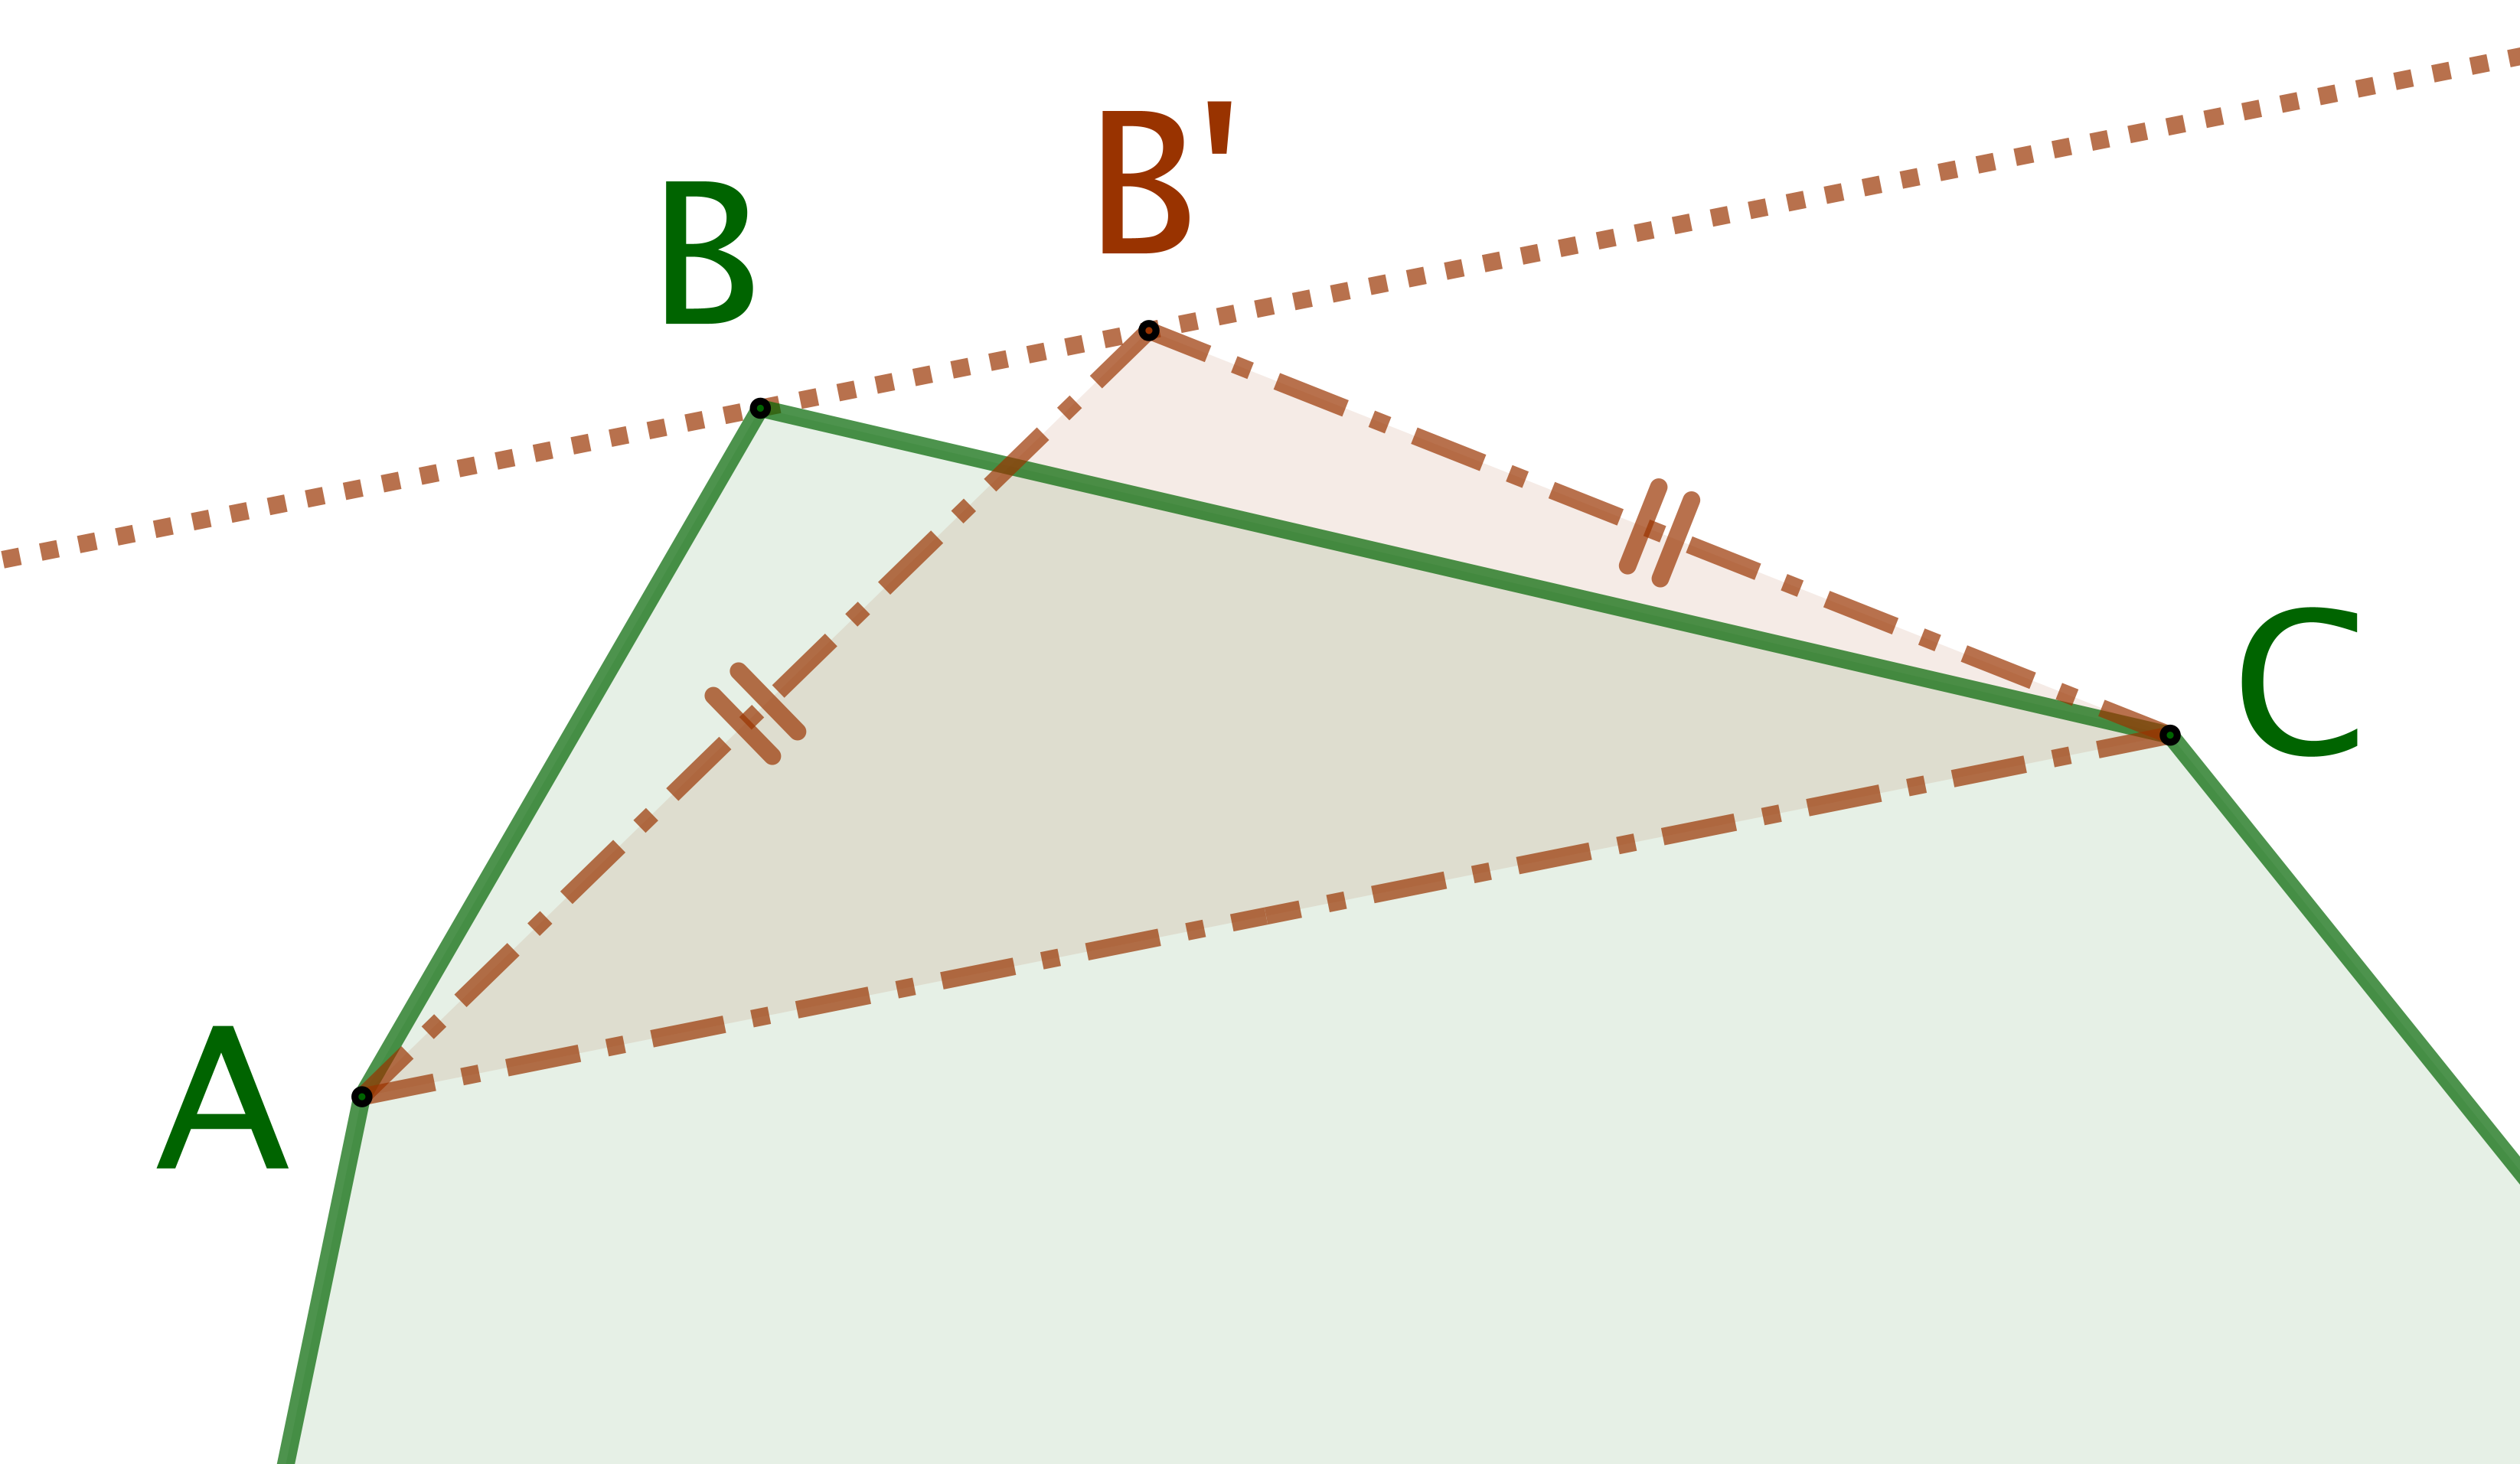
\includegraphics[scale=.4]{content/polygon/sol-must-be/not-iso-OK.png}

		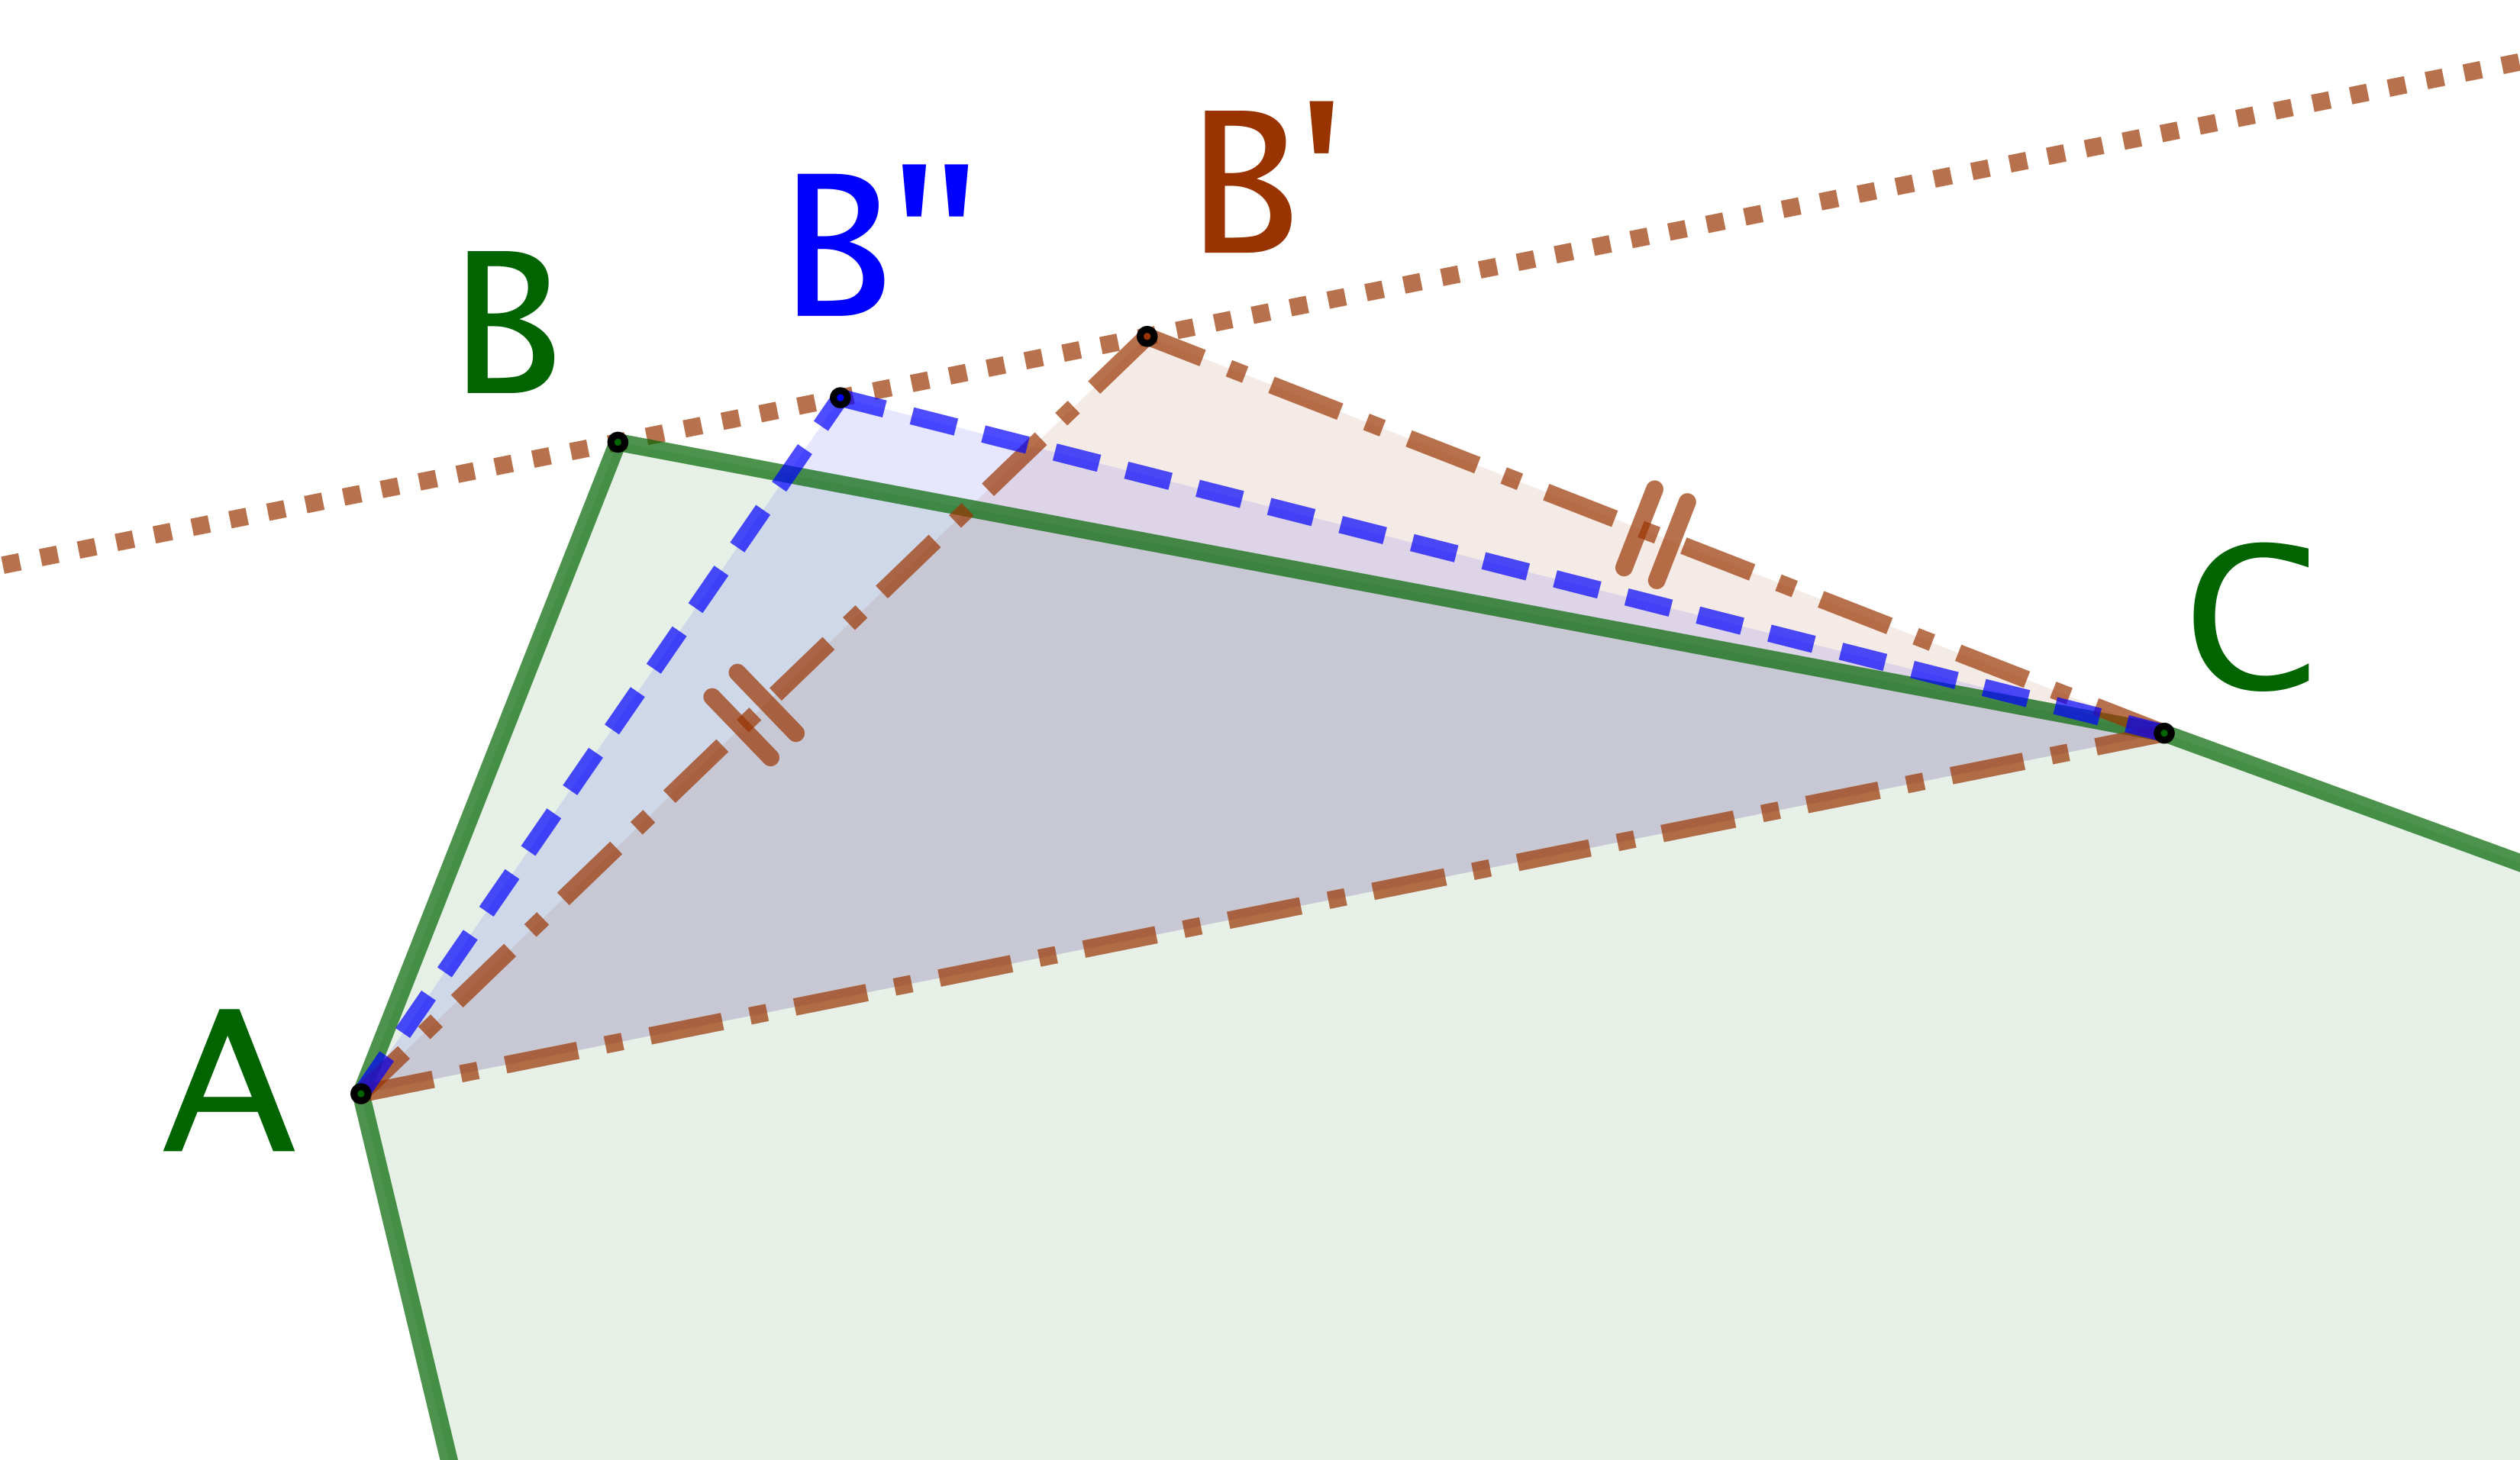
\includegraphics[scale=.4]{content/polygon/sol-must-be/not-iso-KO.png}
	\end{multicols}

	Dans chaque cas, nous avons construit un \ngone\ convexe $\dbleprimeit{\setproba{P}}$ tel que
	$\perim{\dbleprimeit{\setproba{P}}} < \perim{\setproba{P}}$
	et
	$\area{\dbleprimeit{\setproba{P}}} = \area{\setproba{P}}$.
	Une homothétie de rapport $r > 1$, où $r = \frac{ \perim{\setproba{P}} }{ \perim{\setproba{E}} }$, donne un \ngone\ convexe $\primeit{\setproba{P}}$ vérifiant
	$\perim{\primeit{\setproba{P}}} = \perim{\setproba{P}}$
	et
	$\area{\primeit{\setproba{P}}} > \area{\setproba{P}}$.
\end{proof}


\begin{remark}
	Le fait précédent ne permet pas de se ramener toujours au cas d'un \nequi\ convexe. Il nous dit juste que si un \ngone\ convexe maximise son aire à périmètre fixé, alors il devra être, a minima, un \nequi. La nuance est importante, et une similaire existe pour la conclusion du fait suivant.
\end{remark}


% ----------------------- %


\begin{fact} \label{must-be-reg}
	Si un \nequi\ convexe $\setproba{P}$ n'est pas équiangle,
	alors il existe un \ngone\ convexe $\primeit{\setproba{P}}$ tel que
	$\perim{\primeit{\setproba{P}}} = \perim{\setproba{P}}$
	et
	$\area{\primeit{\setproba{P}}} > \area{\setproba{P}}$.
\end{fact}


\begin{proof}
%	Par hypothèse, nous avons deux paires de côtés
%	$\big( [AB] , [BC] \big)$ et
%	$\big( [DE] , [EF] \big)$ telles que
%	$\anglein{BAC} > \anglein{DEF}$ comme ci-dessous, sans savoir si un côté lie les sommets $C$ et $D$, et de même pour $F$ et $A$.
%	Par contre, il est possible que $C$ et $D$ soient confondus.
%	%
%	\begin{multicols}{2}
%		\centering
%		
%		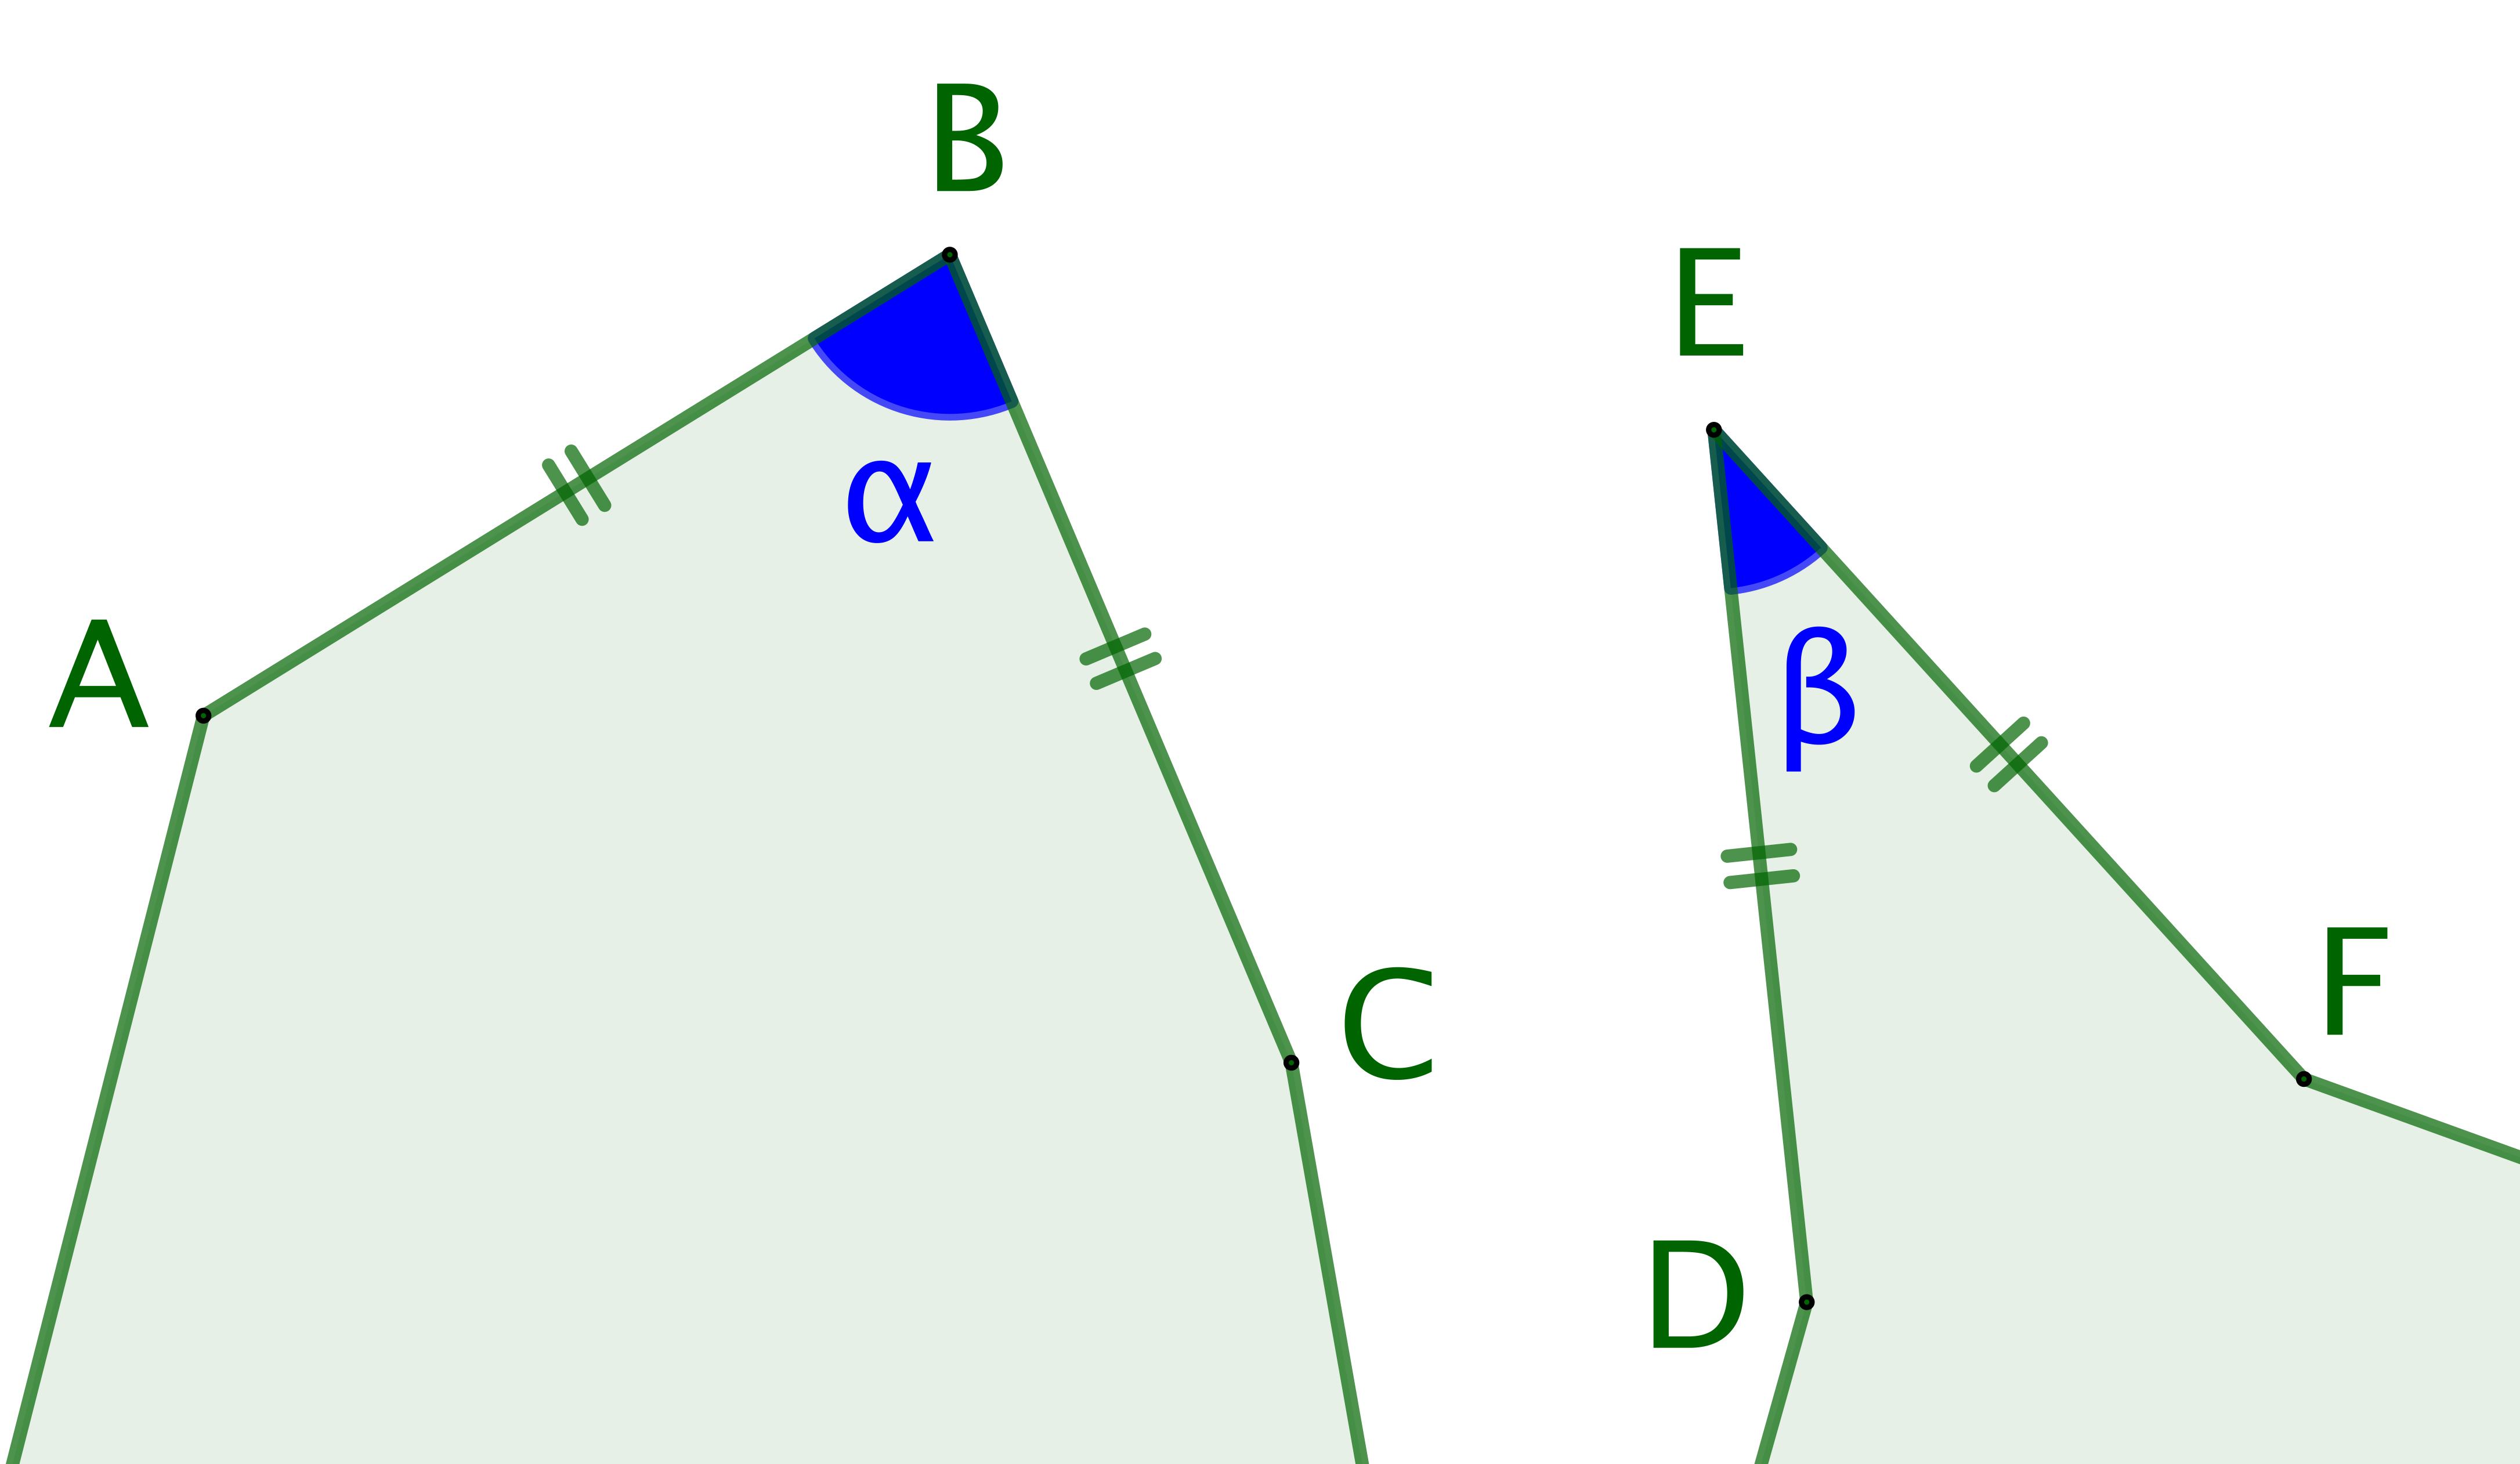
\includegraphics[scale=.4]{content/polygon/sol-must-be/2-eq-angles-start.png}
%		
%		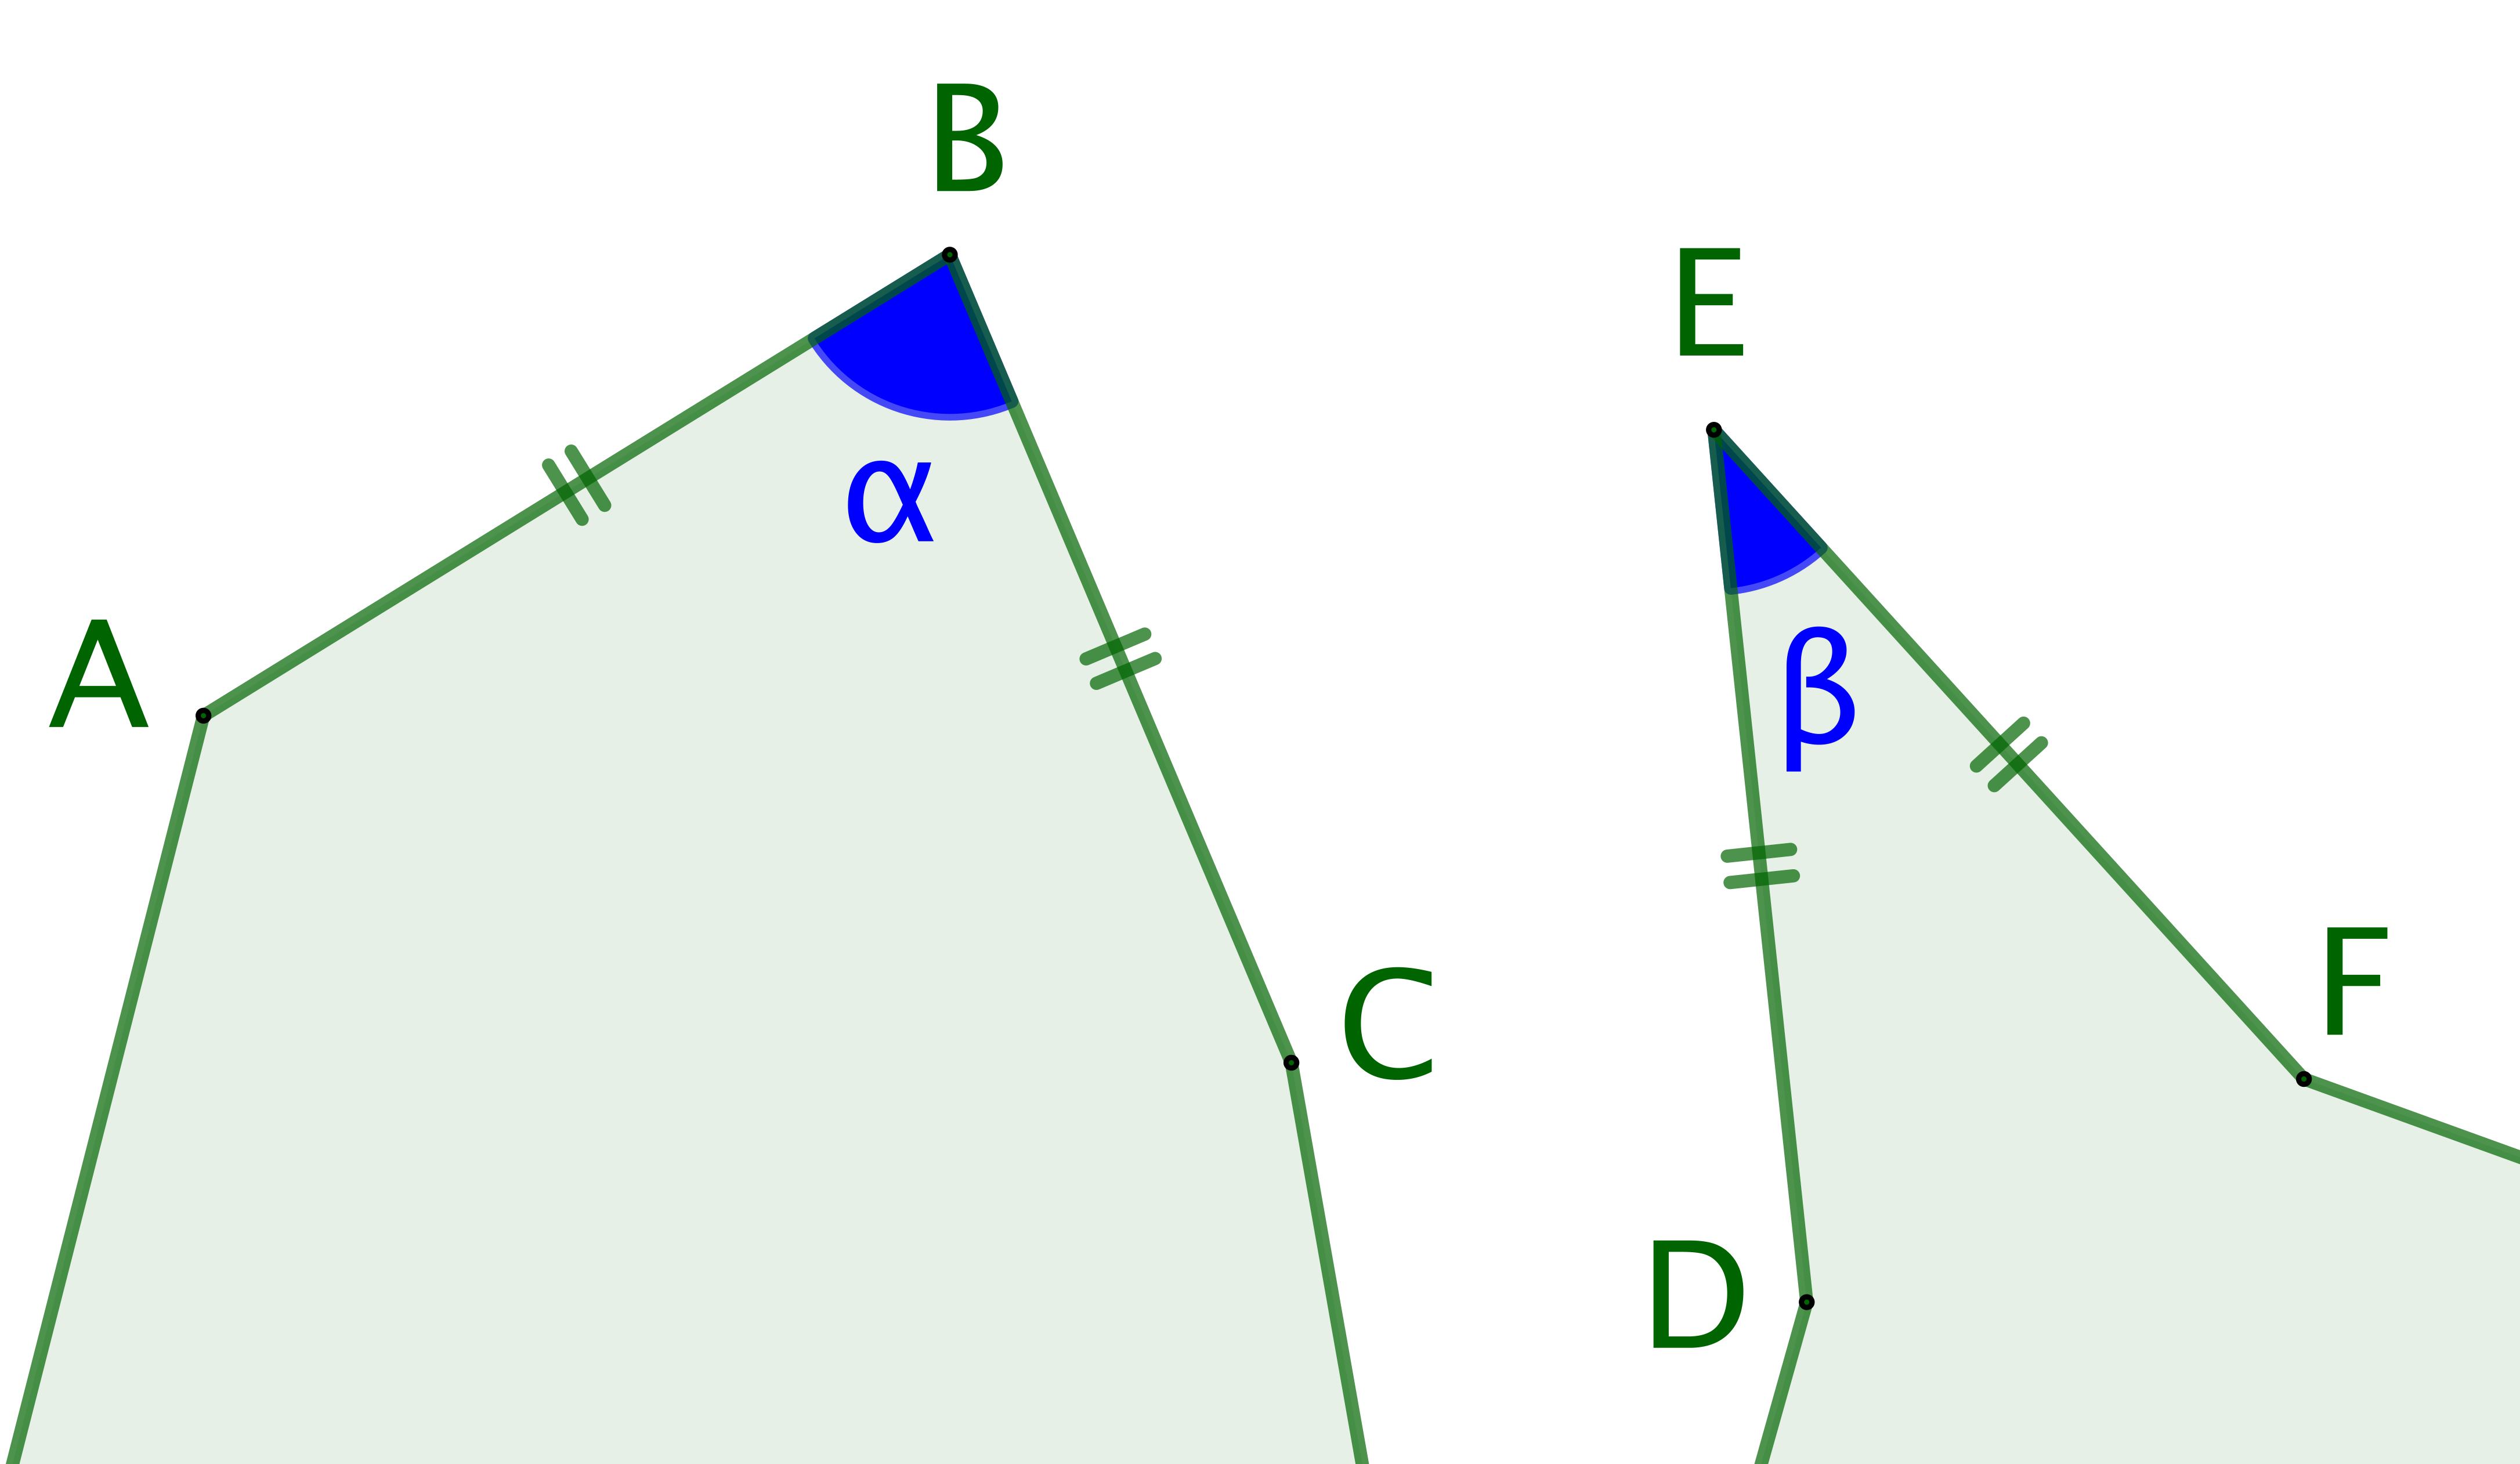
\includegraphics[scale=.4]{content/polygon/sol-must-be/2-eq-angles-start.png}
%	\end{multicols}
%	
%	
%	
%	\newpage
%	
%
%
%
%
%	
%	Dans nos manipulations à venir, nous fixons $A$, $C$, $E$ et $G$, tout en cherchant à bouger $B$ et $F$ de sorte à toujours avoir des triangles isocèles \focus{pointant} vers l'extérieur du convexe $\setproba{P}$.
%	Posons $\ell = AB$, $d_1 = AC$ et $d_2 = EG$. Comme nous ne touchons pas aux points $A$, $C$, $E$ et $G$, les nombres $d_1$ et $d_2$ sont constants.
%	%
%	\begin{itemize}
%		\item ????
%
%		\item ????
%	\end{itemize}
%
%
%	FAUX 
%	Les deux exemples ci-dessus nous permettent de noter que si $\alpha = \anglein{ABC}$ diminue, et $\beta = \anglein{EFG}$ augmente, alors la somme des aires se rapprochent de $0$.
%	Par raison de symétrie, si on fixe $\anglein{ABC} + \anglein{EFG}$, on devine que la somme des aires est maximisée quand $\anglein{ABC} = \anglein{EFG}$.
%	Nous allons établir ceci de façon élémentaire en commençant par les calculs suivants où
%	$\ell = AB$,
%	$\mu = \frac{\alpha + \beta}{2}$ et
%	$\delta = \mu - \beta > 0$ (rappelons que nous avons supposé $\alpha > \beta$).
%
%	\medskip
%	\begin{stepcalc}[style=ar*]
%		\area{ABC} + \area{EFG}
%	\explnext*{Formule dite des sinus.}{}
%		\dfrac12 BA \cdot BC \cdot \sin \big( \anglein{ABC} \big)
%		+
%		\dfrac12 FE \cdot FG \cdot \sin \big( \anglein{EFG} \big)
%	\explnext{}
%		\dfrac12 \ell^2 ( \sin \alpha + \sin \beta )
%	\explnext*{Formules de Simpson.}{}
%		\dfrac12 \ell^2 \sin \big( \dfrac{\alpha + \beta}{2} \big) \cos \big( \dfrac{\alpha - \beta}{2} \big)
%	\explnext{}
%		\dfrac12 \ell^2 \sin \mu \cos \delta
%	\end{stepcalc}
%
%
%	\medskip
%
%	Comme $(\delta ; \mu) \in \intervalO{0}{\pi}^2$,
%	nous avons $\sin \mu \cos \delta > \sin \mu$.
%	Remplaçons alors $\alpha$ et $\beta$ respectivement par $\alph\primeit{A}$ et $\bet\primeit{A}$ de telle sorte que $\alph\primeit{A} = \bet\primeit{A} = \frac{\alpha + \beta}{2} = \mu$.
%	Notons que
%	$0 < \beta < \mu < \alpha < \pi$
%	(diminution de $\alpha$ et augmentation de $\beta$).
%	Deux situations se présentent à nous.
%	%
%	\begin{itemize}
%		\item Le \ngone\ obtenu ne perd aucun côté.
%		Comme la convexité est gardée, c'est gagné.
%
%		\item Le \ngone\ obtenu perd au moins un côté. La solution consiste à choisir
%		$\alpha^{\,\prime\prime} = \mu + \frac{\delta}{2}$ et $\beta^{\,\prime\prime} = \mu - \frac{\delta}{2}$
%		au lieu de
%		$\alph\primeit{A} = \bet\primeit{A} = \mu$, puisque nous avons
%		$\cos \delta < \cos \big( \frac{\delta}{2} \big)$ et
%		$0 < \beta < \beta^{\,\prime\prime} < \mu < \alpha^{\,\prime\prime} < \alpha < \pi$.
%	\end{itemize}
\end{proof}


\begin{remark}
	Une démonstration géométrique courante du fait précédent, que l'on retrouve souvent reproduite, s'appuie sur un résultat attribué à Zénodore sur la maximisation de l'aire totale de deux triangles isocèles de bases fixées, et de périmètre total constant:
	ce résultat affirme que les deux triangles doivent avoir des angles en leur sommet principal de même mesure.
	Malheureusement, cette preuve échoue lors de la disparition d'un sommet en choisissant les deux triangles isocèles optimaux pour construire un nouveau \ngone\ \focus{plus gros}, sauf à affiner la recherche comme dans notre approche analytique.
	Indiquons, au passage, que la preuve du résultat de Zénodore est un peu fastidieuse, sans être ingrate.
\end{remark}
%	
%
%% ----------------------- %
%
%
%%\begin{remark}
%%	La méthode des extrema liés, rappelée dans la remarque \ref{constrained-extrema}, donne une autre justification. Voici comment faire.
%%	%
%%	\begin{itemize}
%%		\item $\area{ABC} + \area{EFG} = \frac14 ( d_1^2 \tan \alpha + d_2^2 \tan \beta )$
%%
%%		\item
%%		\begin{stepcalc}[style=sar]
%%			4 \ell
%%		\explnext{}
%%			AB + BC + EF + FG
%%		\explnext{}
%%			2 ( AB + EF )
%%		\explnext{}
%%			\frac{d_1}{\cos \alpha} + \frac{d_2}{\cos \beta}
%%		\end{stepcalc}
%%
%%		\item Pour $(\alpha ; \beta) \in \intervalO{0}{\frac{\pi}{2}}^2$, on cherche donc à maximiser $f(\alpha ; \beta) =  d_1^2 \tan \alpha + d_2^2 \tan \beta$ sous la contrainte $g(\alpha ; \beta) = 0$ où $g(\alpha ; \beta) = 4 \ell - \frac{d_1}{\cos \alpha} - \frac{d_2}{\cos \beta}$.
%%
%%		\item On doit avoir $\lambda \in \RR$ tel que
%%    	$\pder[i]{f}{\alpha}{1} = \lambda \pder[i]{g}{\alpha}{1}$ et
%%    	$\pder[i]{f}{\beta}{1} = \lambda \pder[i]{g}{\beta}{1}$
%%		(méthode des extrema liés).
%%
%%		\item Donc
%%    	$\frac{d_1^2}{\cos^2 \alpha} = \lambda \frac{d_1 \sin \alpha}{\cos^2 \alpha}$,
%%		c'est-à-dire
%%		$\lambda \sin \alpha = d_1$.
%%		De même,
%%		$\lambda \sin \beta = d_2$.
%%	
%%		\item ????
%%	\end{itemize}
%%\end{remark}


% ----------------------- %


\begin{fact} \label{nece-cond}
	Si un \ngone\ $\setproba{P}$ n'est pas un \nreg\ convexe,
	alors il existe un \ngone\ convexe $\primeit{\setproba{P}}$ tel que
	$\perim{\primeit{\setproba{P}}} = \perim{\setproba{P}}$
	et
	$\area{\primeit{\setproba{P}}} > \area{\setproba{P}}$.
\end{fact}


\begin{proof}
	Il suffit d'utiliser les faits \ref{must-be-conv}, \ref{must-be-equi} et \ref{must-be-reg}.
\end{proof}


% ----------------------- %


Afin d'en finir avec le problème d'isopérimétrie polygonal, nous aurons besoin du fait suivant.


\begin{fact} \label{nregs-sorting}
	Si $\setproba*{R}{1}$ et $\setproba*{R}{2}$ sont respectivement un \xgone{k_1} et un \xgone{k_2}, tous les deux réguliers convexes, avec 
	$k_1 < k_2$ et $\perim{\setproba*{R}{1}} = \perim{\setproba*{R}{2}}$,
	alors
	$\area{\setproba*{R}{1}} < \area{\setproba*{R}{2}}$.
\end{fact}


\begin{proof}
    Il est connu, et facile de démontrer, qu'un \nreg\ convexe $\setproba{R}$ vérifie
    $\perim{\setproba{R}} = 2 n \sin (\frac{\pi}{n}) \rho$
    et
	$\area{\setproba{R}} = n \sin (\frac{\pi}{n})  \cos (\frac{\pi}{n}) \rho^2$
	où $\rho$ désigne le rayon du cercle circonscrit à $\setproba{R}$.
	Ceci donne 
	$\area{\setproba{R}} = \frac{\perim{\setproba{R}}^2}{4 n \tan (\frac{\pi}{n})}$,
	puis amène à justifier que 
	$k_1 \tan (\frac{\pi}{k_1}) > k_2 \tan (\frac{\pi}{k_2})$.
	Donc, nous devons démontrer que la suite $\big( k \tan (\frac{\pi}{k}) \big)_{k \in \leq 3}$ est strictement décroissante.
	
	
	XXXX
\end{proof}

